\documentclass{report}
\usepackage[T1]{fontenc}
\usepackage[utf8]{inputenc}
\usepackage[backend=biber, style=ieee]{biblatex}
\usepackage{csquotes}
\usepackage[portuguese]{babel}
\usepackage{blindtext}
\usepackage[printonlyused]{acronym}
\usepackage{hyperref}
\usepackage{graphicx}
\usepackage{indentfirst}
\usepackage{float}
\bibliography{bibliografia}

\begin{document}
%%% DEFINIÇÕES GLOBAIS %%%
\def\titulo{Realidade Aumentada}
\def\data{Aveiro, dezembro 2021}
\def\autores{Miguel Vila, Diogo Silva}
\def\autorescontactos{(107276) miguelovila@ua.pt, (108212) dsgps@ua.pt}
\def\versao{BETA SINCE 2013}
\def\departamento{DETI}
\def\empresa{UNIVERSIDADE DE AVEIRO}
\def\logotipo{ua.pdf}

%%% ESTRUTURA CAPA %%%
\begin{titlepage}
\begin{center}
\vspace*{50mm}
{\Huge \titulo}\\ 
\vspace{10mm}
{\Large \empresa}\\
\vspace{10mm}
{\LARGE \autores}\\ 
\vspace{30mm}
\begin{figure}[h]
\center
\includegraphics{\logotipo}
\end{figure}
\vspace{30mm}
\end{center}
\begin{flushright}
\versao
\end{flushright}
\end{titlepage}

%%%  PÁGINA DE TÍTULO %%%
\title{%
{\Huge\textbf{\titulo}}\\
{\Large \departamento\\ \empresa}
}
\author{
    \autores \\
    \autorescontactos
}
\date{\data}
\maketitle
\pagenumbering{roman}

%%% RESUMO %%%
\begin{abstract}
!!!TODO!!! Resumo de 200-300 palavras.
\end{abstract}

%%% AGRADECIMENTOS %%%
\renewcommand{\abstractname}{Agradecimentos}
\begin{abstract}
!!!TUDO!!!
\end{abstract}

\tableofcontents
% \listoftables
% \listoffigures

\clearpage
\pagenumbering{arabic}

%%% INTRODUÇÃO %%%%
\chapter{Introdução}
\label{chap.introducao}
Desde os primórdios que o Homem procura ter controlo da sua realidade moldando-a e modificando-a de modo a que as suas necessidades sejam supridas. Pode-se tomar como exemplo o controlo do fogo: quando o Homem primitivo descobriu como gerar artificialmente e controlar o fogo teve a sua vida facilitada e abriu um leque de novas possibilidades que originaram uma grande revolução a todos os níveis.

Passados alguns milhares de anos, o ser humano continua a tentar ter ainda mais controlo sobre a realidade de modo a que o impossível se torne possível. Como a \ac{ra} estende virtualmente aquilo que existe no mundo real, existe uma forte probabilidade de que, tal como o fogo, a \ac{ra} venha a revolucionar a forma como se vive e dar azo ao surgimento de novas possibilidades.

Apesar de ser uma tecnologia relativamente recente, esta tem tido uma considerável evolução por isso, promete ser o futuro da tecnologia e integrar-se cada vez mais no dia a dia do cidadão comum. Atualmente não está implementada em grande escala, mas já tem vastas aplicações a nível empresarial. Áreas como a medicina, o entretenimento, o \textit{design}, a educação e a arquitetura poderão beneficiar dos novos recursos e funcionalidades criados por esta tecnologia.

Além disso, empresas no mercado tecnológico como a Google, a Microsoft e a Samsung apostam no desenvolvimento desta tecnologia que tem potencial para se tornar o “braço-direito” do utilizador no desenvolver da sua atividade profissional e, futuramente, no desenvolvimento da sua vida pessoal. Porém, atualmente apenas a Microsoft foi capaz de, com algum sucesso, viabilizar e introduzir estes dispositivos no ambiente industrial e corporativo.

Será que, com todo este investimento e interesse por parte de grandes empresas tecnológicas, esta tecnologia estará à altura para mudar o mundo num futuro próximo?

\section{Objetivos}
Este relatório, realizado no âmbito da unidade curricular de Introdução à Engenharia Informática, terá como principal objetivo dar a conhecer a nova realidade tecnológica dos dispositivos \textit{mixed reality} e a sua utilidade, focando nos óculos holográficos de realidade aumentada \textit{HoloLens 2} desenvolvidos pela Microsoft.

Tentar-se-á ainda responder a algumas perguntas frequentes quando o assunto é \ac{ra} tais como: "Será que a \ac{ra} é uma tecnologia relevante?", "A \ac{ra} surgirá no nosso quotidiano num futuro próximo?" e "Quais são as limitações atuais desta tecnologia?"

\section{Organização e estrutura}
O relatório \textit{Realidade Aumentada} contém informação abrangente relativa a esta área e está organizado de forma a que o leitor não necessite de quaisquer conhecimentos prévios para poder acompanhar a totalidade dos capítulos.

O documento encontra-se dividido em 5 capítulos:
\begin{itemize}
    \item No \autoref{chap.introducao} é feita a contextualização do trabalho, explicando o porquê da \ac{ra} ser um tema importante e de interesse. Também são explicitados os objetivos que se pretendem atingir com a leitura do mesmo.
    \item No \autoref{chap.realidade-aumentada} ir-se-á esclarecer o que é a \ac{ra}, perceber como surgiu e ainda explorar possíveis aplicações e alguns exemplos de como a \ac{ra} já está a ser utilizada no quotidiano.
    \item No \autoref{chap.oculos-holograficos} é explicado o conceito por detrás dos óculos holográficos. Também se faz um balanço do panorama atual desses dispositivos.
    \item No \autoref{chap.microsoft-hololens-2} analisa-se em detalhe os óculos de realidade aumentada \textit{HoloLens 2} percebendo qual a sua utilidade, quais as suas principais características e a quem se destina.
    \item Por fim, no \autoref{chap.conclusao} serão apresentadas as principais conclusões do trabalho, prevendo de que forma esta tecnologia irá revolucionar e entrar nas vidas do cidadão comum.
\end{itemize}

\section{Metodologia}
Para o presente trabalho, foi utilizada uma metodologia assente na pesquisa exploratória. Esta pesquisa de índole qualitativa baseou-se na recolha de dados em diferentes fontes, tais como revistas de referência na área da tecnologia e ciência e investigações/estudos nestas mesmas áreas.

A informação daí recolhida permitiu compreender, aprofundar e consolidar o tema do trabalho, de maneira a apresentá-lo da forma mais clara mais objetiva possível.

%%% REALIDADE AUMENTADA %%%
\chapter{Realidade Aumentada}
\label{chap.realidade-aumentada}
Neste capítulo irá se explicar em que consiste a \ac{ra}, diferenciando-a de tecnologias semelhantes como a \ac{rv} e apresenta-se as diferentes aplicações que a \ac{ra} já tem no quotidiano e que, por muitas vezes, passam despercebidas.

Mostrar-se-á também a sua origem e as diversas etapas que teve que atravessar ao longo dos anos para se tornar na tecnologia que é hoje. Por fim, apresenta-se alguns exemplos de aplicações no mundo real e exemplos de dispositivos inteligentes que possuem esta tecnologia.

\section{Conceito}
A \ac{ra} consiste na integração e interligação de elementos ou informações virtuais na visualização do mundo real. É através de dispositivos de entrada como sensores óticos (câmera) e sensores de movimento (giroscópio e acelerómetro) e dispositivos de saída como um écran (convencional ou holográfico) que é feita essa integração do virtual com mundo palpável.

A \ac{ra} é comumente confundida com a \ac{rv} porque, a princípio, podem parecer tecnologias semelhantes, mas, na verdade, existem diversas diferenças entre elas.

Enquanto que a \ac{rv}, tal como o nome indica, pode ser caracterizada pela criação de um ambiente puramente virtual onde o utilizador tenta ter uma experiência imersiva, a \ac{ra} trata-se de uma tecnologia que, através de dispositivos especificos, permite que elementos virtuais interliguem-se e, até mesmo, interajam com a realidade.

Por outras palavras, a \ac{ra} baseia-se numa experiência interativa entre o mundo real e o virtual, onde objetos que pertencem ao plano real podem ser "aumentados" e manipulados no plano virtual e onde objetos pertencentes ao plano virtual podem interagir e moldar-se ao mundo físico.

A \ac{ra} é uma tecnologia abrangente e cheia de possibilidades, por isso, ainda pode ser subdividida em duas outras: a Realidade Mediada e a \ac{rm}. Estas são semelhantes no que toca àquilo que pretendem alcançar, porém usam diferentes técnicas para o fazer:
\begin{itemize}
    \item Na Realidade Mediada, uma câmera capta o ambiente que envolve o utilizador, as imagens obtidas são processadas inserindo os elementos virtuais e, por fim, a imagem é mostrada num écran.
    \item Na \ac{rm}, uns sensores óticos e posicionais mapeiam o ambiente ao redor do utilizador, as posições em que os objetos virtuais aparecerão são processadas e, por fim, os objetos são projetados numa lente transparente dando a noção de profundidade, culminando, assim, numa experiência ainda mais real e imersiva para o utilizador.
\end{itemize}

\begin{figure}[H]
    \centering
    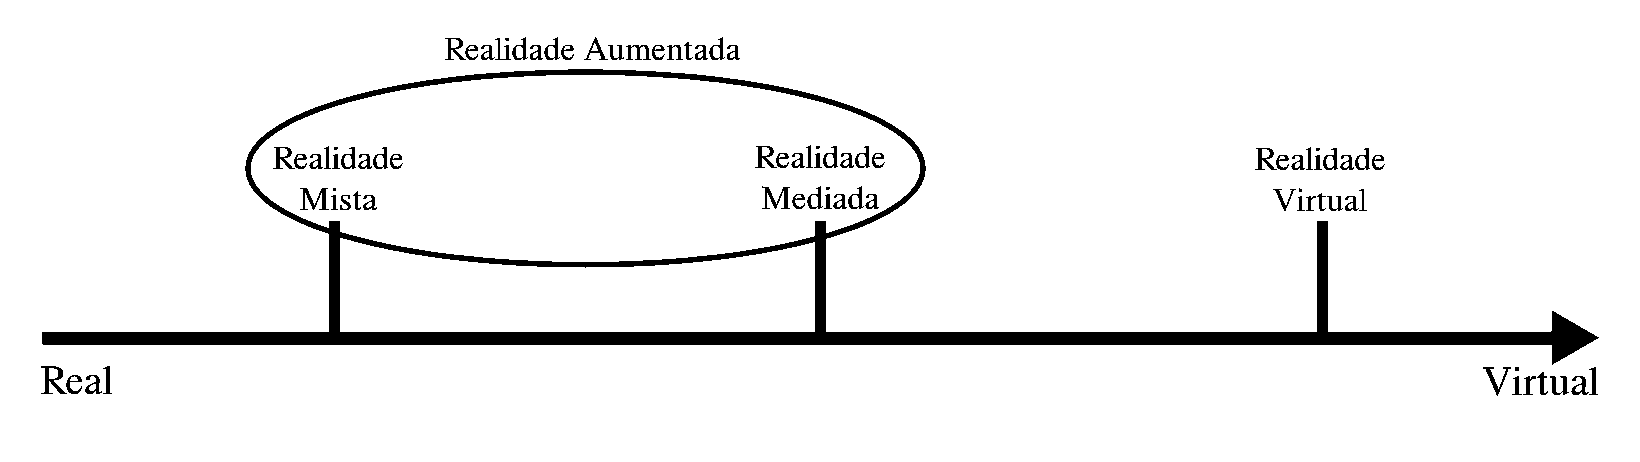
\includegraphics[width=\textwidth]{spectre.png}
    \caption{Espetro de proximidade ao real ou virtual.}
    \label{Fig:DesktopSpotify}
\end{figure}

Conclui-se então que a \ac{ra} está mais próxima do real do que a \ac{rv} já que esta cria um ambiente totalmente virtual praticamente dissociado do mundo palpável. Conclui-se também que entre a Realidade Mediada e a \ac{rm} esta é aquela que confere um maior grau de imersividade ao utilizador.

\section{Origem}
A primeira referência ao conceito de Realidade Aumentada remonta ao ano de 1962 quando Morton Heilig construiu uma máquina com tecnologia multisensorial imersiva que denominou de Sensorama.

Esta máquina oferecia uma experiência de \ac{ra} multisensorial imersiva já que era capaz de exibir imagens em 3D, som estéreo, sensações hápticas através da inclinação do corpo, sensações de vento e aromas.

Em 1968, Ivan Sutherland desenvolveu o primeiro \ac{hmd} a que chamou \textit{The Sword of Damocles}, que é um dispositivo usado na cabeça, parte integrante de um capacete, que possui um display óptico em frente de um (\ac{hmd} Monocular) ou de cada olho (\ac{hmd} Binocular).

Apesar do conceito já existir há imenso tempo, o termo Realidade Aumentada só foi criado em 1992 pelo investigador Tom Caudell da Boeing. Ele e o seu colega David Mizell tiveram o desafio de fornecer uma alternativa aos diagramas e dispositivos de marcação usados para guiar os trabalhadores no chão de fábrica da empresa. A solução que desenvolveram foi um \ac{hmd} que poderia ser usados pelos trabalhadores e exibia os diagramas e esquemas dos aviões e os projetava em placas reutilizáveis, sendo que a informação a visualizar poderia ser alterada através de computador.

\section{Aplicações}
Ao contrário do que muitos podem imaginar, a realidade aumentada não se limita apenas ao contexto de empresas de tecnologia — as aplicações e softwares desenvolvidos têm utilidade nas mais variadas situações do nosso dia a dia.

Por esse motivo o uso desta ferramenta está principalmente presente:

Nos Jogos - Na área dos jogos, a realidade aumentada oferece um vasto leque para se explorar a criatividade e levar experiências únicas aos seus usuários — é uma forma, inclusive, de fazer as pessoas saírem do sedentarismo e ao mesmo tempo ter uma fonte de diversão.

Na Medicina - A aplicação da realidade aumentada também já alcançou um papel de destaque na medicina. Fazendo com que, seja possível projetar o corpo humano com os seus órgãos e sistemas, de maneira que o profissional tenha uma visão mais clara e precisa de todos, bem como a melhor medida a ser adotada mediante casos práticos.Uma grande vantagem gerada para o cenário médico é a segurança para os procedimentos de uma forma geral: cirurgias, atendimentos clínicos e exames, sem deixar de mencionar a parte dos estudos.

Na Arquitetura - Na arquitetura, contar com os recursos da realidade aumentada pode facilitar bastante a prestação do serviço, sobretudo na fase de construção dos projetos. Atualmente, já existem equipamentos que conseguem, por exemplo, fazer a medida de determinado local digitalmente, possibilitando que esses dados sejam acessados por computadores e tablets. Com o auxílio dessa ferramenta, os arquitetos têm a oportunidade de criar imagens realistas em 3D,  não apenas da planta da obra, mas dos ambientes individuais, de forma que o cliente tenha uma percepção mais clara da expectativa de resultado final. É um instrumento que vai potencializar o trabalho do profissional e, ao mesmo tempo, possibilitar uma melhor partilha de ideias com os destinatários dos seus serviços.

Na Indústria - Com tendência forte no mercado, a indústria já representa uma forma de atuar totalmente tecnológica e inovadora, visto que tem como base sistemas que conectam toda a sua linha de produção e viabilizam a coleta de informações em tempo real. O que a realidade aumentada vem a acrescentar a esse contexto é a simulação de um processo em 3D ainda na fase de testes, ou seja, antes de colocá-lo em prática definitivamente. Outras perspectivas das aplicações de realidade aumentada na indústria são os tutoriais interativos para os setores de inspeção e manutenção. Assim, os funcionários podem contar com uma ajuda interativa sobre o passo a passo para executar o trabalho necessário em cada máquina.

O uso mais utilizado, e mais conhecido da realidade aumentada é o entretenimento, através dos filtros para fotos em aplicativos móveis de redes sociais, através de jogos como o Pokémon GO. A realidade aumentada é também utilizada de muitas formas nas áreas do ensino, design de produtos, ações de marketing, suporte em plantas industriais, entre outros. O uso de vídeos transmitidos ao vivo digitalmente processados e "ampliados" pela adição de gráficos criados pelo computador também podem ser considerados como um tipo de realidade aumentada. Um usuário da \ac{ra} pode utilizar uns óculos, ou câmeras acopladas a um dispositivo computacional, e através destes, poderá ver o mundo real bem como imagens geradas por computador projetadas no mundo.

\subsection{Exemplos}
O nosso telemóvel, com a grande qualidade das câmaras que o integram, a precisão dos sensores (giroscópio e magnetómetro) e, também, com o crescente poder de processamento, tornou-se no equipamento ideal e mais conveniente para fazer uso da realidade aumentada.

Jogos simples como o famoso “Pokémon GO” ou até mesmo aplicações de grandes superfícies como o IKEA aproveitam-se dos potenciais desta tecnologia. No jogo Pokémon GO podemos, por exemplo, “capturar” um Pokémon em três dimensões no ambiente real que rodeia o utilizador. Já na aplicação do IKEA, a realidade
aumentada permite que o utilizador possa experimentar, por exemplo, um móvel que quer comprar no próprio local.

Esta “mesclagem” da realidade com o virtual será visualizada pelo utilizador no próprio display do smartphone. Mas de que forma e com que hardware poderemos ter uma experiência mais real e imersiva?

%%% ÓCULOS HOLOGRÁFICOS %%%
\chapter{Óculos Holográficos}
\label{chap.oculos-holograficos}
!!!TUDO!!!

\section{Conceito}
O conceito de óculos holográficos surgiu exatamente com a criação do conceito de realidade aumentada por Thomas Caudell.

O objetivo dos avanços tecnológicos é fazer com que estes óculos, no futuro, se pareçam bastante com óculos comuns, mas que, nas suas lentes seja apresentada uma
imagem holográfica que se funda com o ambiente real.

\section{Panorama atual}
Esta tecnologia tem vindo a ser alvo de estudo por parte de grandes empresas no ramo da tecnologia que a pretendem implementar em diversas áreas, sejam estas no ramo da engenharia, da saúde, da arquitetura e até da educação.

Toda esta pesquisa levou ao desenvolvimento de hardware específico para que, de forma intuitiva e prática, fosse possível usar a realidade aumentada como “braço-direito” nas tarefas do quotidiano no trabalho. Assim, empresas como a Epson, a Vuzix, a Solos, a Google, a Microsoft, entre outras, têm vindo a desenvolver óculos que permitem ao utilizador utilizar a realidade aumentada na sua atividade profissional. Com tanta pesquisa e com tantas grandes empresas envolvidas, as opções de equipamentos que permitem visualizar a realidade aumentada são bastantes, porém, neste trabalho iremos dar especial atenção aos “Microsoft HoloLens”, o produto de realidade aumentada da Microsoft.

%%% MICROSOFT HOLOLENS 2 %%%
\chapter{Microsoft \textit{HoloLens 2}}
\label{chap.microsoft-hololens-2}
!!!TODO!!!

\section{Proposta do produto}
A Microsoft apresenta ao público um novo e revolucionário dispositivo de realidade aumentada. Através de um design minimalista e moderno, o “HoloLens 2” promete ser mais eficiente que a sua versão anterior e que todos os seus concorrentes.

“Não existirá nenhum produto que compita com o nosso nos próximos dois a três anos e que possa garantir o nível de fidelidade que apresentamos.” (Zulfi Alan, general manager on optics engineering)

\section{Design e principais características}
a. Campo de visão
Uma das maiores críticas direcionadas à primeira versão destes óculos estava relacionada com o pequeno campo de visão. Assim, a segunda versão foi desenhada para permitir apresentar um maior campo de visão aumentando, então, a “imersão” neste ambiente misto.

b. Resolução
Visto que o objetivo de produtos como este prende-se pela inserção de elementos virtuais na realidade existiu a grande necessidade de aumentar a resolução dos hologramas. Assim, através de uma complexa projeção a laser que guia a luz diretamente para a retina do utilizador, o \textit{“display”} transparente emite uma imagem holográfica de resolução 2K em cada um dos olhos do utilizador fazendo com que os hologramas parecem mais naturais e reais.

c. Ajuste interpupilar
Cada pessoa tem características faciais diferentes o que implica a necessidade de um ajuste de forma a que a imagem fique adequada e não cause desconforto ao utilizador. Os HoloLens recorrem a pequenos sensores no interior dos óculos para medir a distância entre as pupilas dos nossos olhos de modo a que então a imagem seja corretamente ajustada.

d. \textit{“Mixed Reality”}
\textit{Mixed Reality} é segundo a Microsoft o termo mais correto para caracterizar o tipo de \ac{ra} a que estes óculos se destinam: uma realidade onde os elementos virtuais se encontram perfeitamente integrados. Com pequenos sensores posicionados nos óculos e através de um sistema de localização e análise dos movimentos das mãos do utilizador é possível manipular os hologramas de forma intuitiva. Para além disto, um algoritmo de inteligência artificial analisa todo o cenário em redor do utilizador e identifica todos os elementos presentes na sala permitindo que o computador identifique superfícies e locais onde poderá ou não projetar um holograma.


\section{Público Alvo}
O grande propósito destes óculos é o aumento da produtividade de cada uma das pessoas que os utiliza.
Para pessoas comuns, este produto poderá ter pouca ou nenhuma utilidade, mas, por outro lado, engenheiros e artistas, por exemplo, podem ver este produto como uma ferramenta muito promissora que poderá facilitar o processo de criação de algo.

%%% CONCLUSÕES %%%
\chapter{Conclusões}
\label{chap.conclusao}
Neste trabalho desenvolvemos e explicamos o conceito de \ac{ra} através da comparação desta tecnologia com a \ac{rv}, da explicação da sua origem e as eventuais utilizações que esta tem e terá no nosso mundo. Apresentamos um dos dispositivos de \ac{ra} mais promissores na atualidade (Óculos Holográficos) exemplificando diversas utilidades práticas que estes têm. Por fim analisamos e demonstramos o produto atual de \ac{ra} que consideramos ser o mais revolucionário, os “Microsoft \textit{HoloLens 2}”. Este foi um trabalho que nos permitiu descobrir e desvendar o atual paradigma desta tecnologia e da qual nos consideramos fãs. Foi possível ainda perceber as limitações da \ac{rv} em relação ao mundo real e concluir que o futuro apresenta-se muito mais promissor para a \ac{ra}. Acreditamos que com a aposta de grandes empresas como a Google e a Microsoft na \ac{ra}, em um curto espaço de tempo, a maioria das atividades comerciais irão fazer uso desta tecnologia. Dado isto não será improvável o surgimento de novas empresas e novos produtos que irão concorrer frente a frente com os que já existem atualmente, permitindo um desenvolvimento ainda maior desta tecnologia fazendo ainda com que num futuro próximo, a utilização desta tecnologia possa vir a ser utilizada no quotidiano de pessoas comuns e não apenas no ambiente corporativo.

\chapter*{Contribuições dos autores}
!!!TODO!!! Ambos participámos ativamente e com empenho, procurando contribuir para a realização dum trabalho com boa apresentação e conteúdo.

Resumir aqui o que cada autor fez no trabalho. Usar abreviaturas para identificar os autores, por exemplo AS para António Silva. No fim indicar a percentagem de contribuição de cada autor.

%%% ACRÓNIMOS %%%
\chapter*{Acrónimos}
\begin{acronym}
\acro{ua}[UA]{Universidade de Aveiro}
\acro{leci}[LECI]{Licenciatura em Engenharia de Computadores e Informática}
\acro{ra}[RA]{Realidade Aumentada}
\acro{rv}[RV]{Realidade Virtual}
\acro{rm}[RM]{Realidade Mista}
\acro{hmd}[HMD]{\textit{head mouted display}}
\end{acronym}

%%% BIBLIOGRAFIA %%%
\printbibliography

https://ccg.pt/realidade-aumentada-aplicabilidade/

https://blog.cronapp.io/realidade-aumentada-e-suas-aplicacoes/

\end{document}